% The LLM-agent MBSE workflow of this repository, in three figures.
% Build: lualatex workflow.tex   (fontspec: Noto Sans Condensed, IBM Plex Mono)
%
% Coordinates are in the units of the published page's SVG (1 unit = 0.03 cm,
% y growing downwards), so the two drawings can be compared point by point.
\documentclass[10pt]{article}
\usepackage[a3paper,landscape,margin=14mm]{geometry}
\usepackage{fontspec}
\setmainfont{Noto Sans Condensed}[BoldFont={Noto Sans Condensed SemiBold}, ItalicFont={Noto Sans Condensed Italic}]
\setmonofont{IBM Plex Mono}[Scale=0.92]
\usepackage{xcolor}
\usepackage{tikz}
\usetikzlibrary{arrows.meta,shapes.geometric,calc}
\usepackage{caption}
\captionsetup{font={small}, labelfont=bf, justification=raggedright, singlelinecheck=false}
\pagestyle{empty}
\setlength{\parindent}{0pt}

% Role colours: what does the work.
\definecolor{ink}{HTML}{17212B}
\definecolor{muted}{HTML}{56636C}
\definecolor{rule}{HTML}{C8D0D2}
\definecolor{faint}{HTML}{E9EDED}
\definecolor{agent}{HTML}{B8470F}
\definecolor{agentTint}{HTML}{F6E4D8}
\definecolor{script}{HTML}{46596B}
\definecolor{scriptTint}{HTML}{E1E7EC}
\definecolor{check}{HTML}{0B6E66}
\definecolor{checkTint}{HTML}{D9EEEA}
\definecolor{human}{HTML}{7A3E8C}
\definecolor{humanTint}{HTML}{EFE2F2}

\tikzset{
  px/.style={x=0.03cm, y=-0.03cm},
  agent/.style={draw=agent, fill=agentTint, line width=0.8pt, rounded corners=2.5pt},
  script/.style={draw=script, fill=scriptTint, line width=0.8pt, rounded corners=1.5pt},
  check/.style={draw=check, fill=checkTint, line width=0.8pt, rounded corners=1.5pt},
  model/.style={draw=ink, fill=white, line width=0.8pt, rounded corners=1pt},
  record/.style={draw=muted, line width=0.5pt, dash pattern=on 1.5pt off 2pt, rounded corners=2pt},
  gate/.style={diamond, draw=human, fill=humanTint, line width=0.8pt, inner sep=0pt, minimum size=#1},
  gate/.default=36pt,
  gatedash/.style={gate=#1, dash pattern=on 3pt off 2pt},
  gatedash/.default=31pt,
  flow/.style={draw=ink, line width=0.7pt, -{Stealth[length=5pt,width=4pt]}},
  flowagent/.style={draw=agent, line width=0.9pt, -{Stealth[length=5pt,width=4pt]}},
  flowcheck/.style={draw=check, line width=0.9pt, -{Stealth[length=5pt,width=4pt]}},
  flowhuman/.style={draw=human, line width=0.8pt, dash pattern=on 3pt off 2.5pt, -{Stealth[length=5pt,width=4pt]}},
  flowfaint/.style={draw=muted, line width=0.6pt, dash pattern=on 2pt off 2pt, -{Stealth[length=4pt,width=3.5pt]}},
  t/.style={inner sep=0pt, anchor=base, font=\fontsize{9}{11}\selectfont, text=ink},
  tl/.style={t, anchor=base west},
  tr/.style={t, anchor=base east},
  tm/.style={t, font=\fontsize{10.5}{12}\selectfont},
  tb/.style={t, font=\fontsize{10.5}{12}\selectfont\bfseries},
  th/.style={t, font=\fontsize{12}{14}\selectfont\bfseries},
  thl/.style={th, anchor=base west},
  tmu/.style={t, text=muted},
  tmul/.style={tl, text=muted},
  tmono/.style={t, font=\ttfamily\fontsize{8}{10}\selectfont, text=muted},
  tmonol/.style={tmono, anchor=base west},
  band/.style={inner sep=0pt, anchor=base west, font=\fontsize{9}{11}\selectfont\bfseries, text=muted},
  bandsub/.style={inner sep=0pt, anchor=base west, font=\fontsize{7.5}{9}\selectfont, text=muted},
}

\begin{document}

% ───────────────────────────── Figure 1 ─────────────────────────────
{\fontsize{24}{28}\selectfont\bfseries Gated Layered Workflow}\par\smallskip
{\color{muted}A brief goes in; one checked SysML-like model comes out, layer by layer. Language models write each layer, scripts carry what one layer owes the next, and a Sysprose check holds every step before the run moves on.}\par\medskip

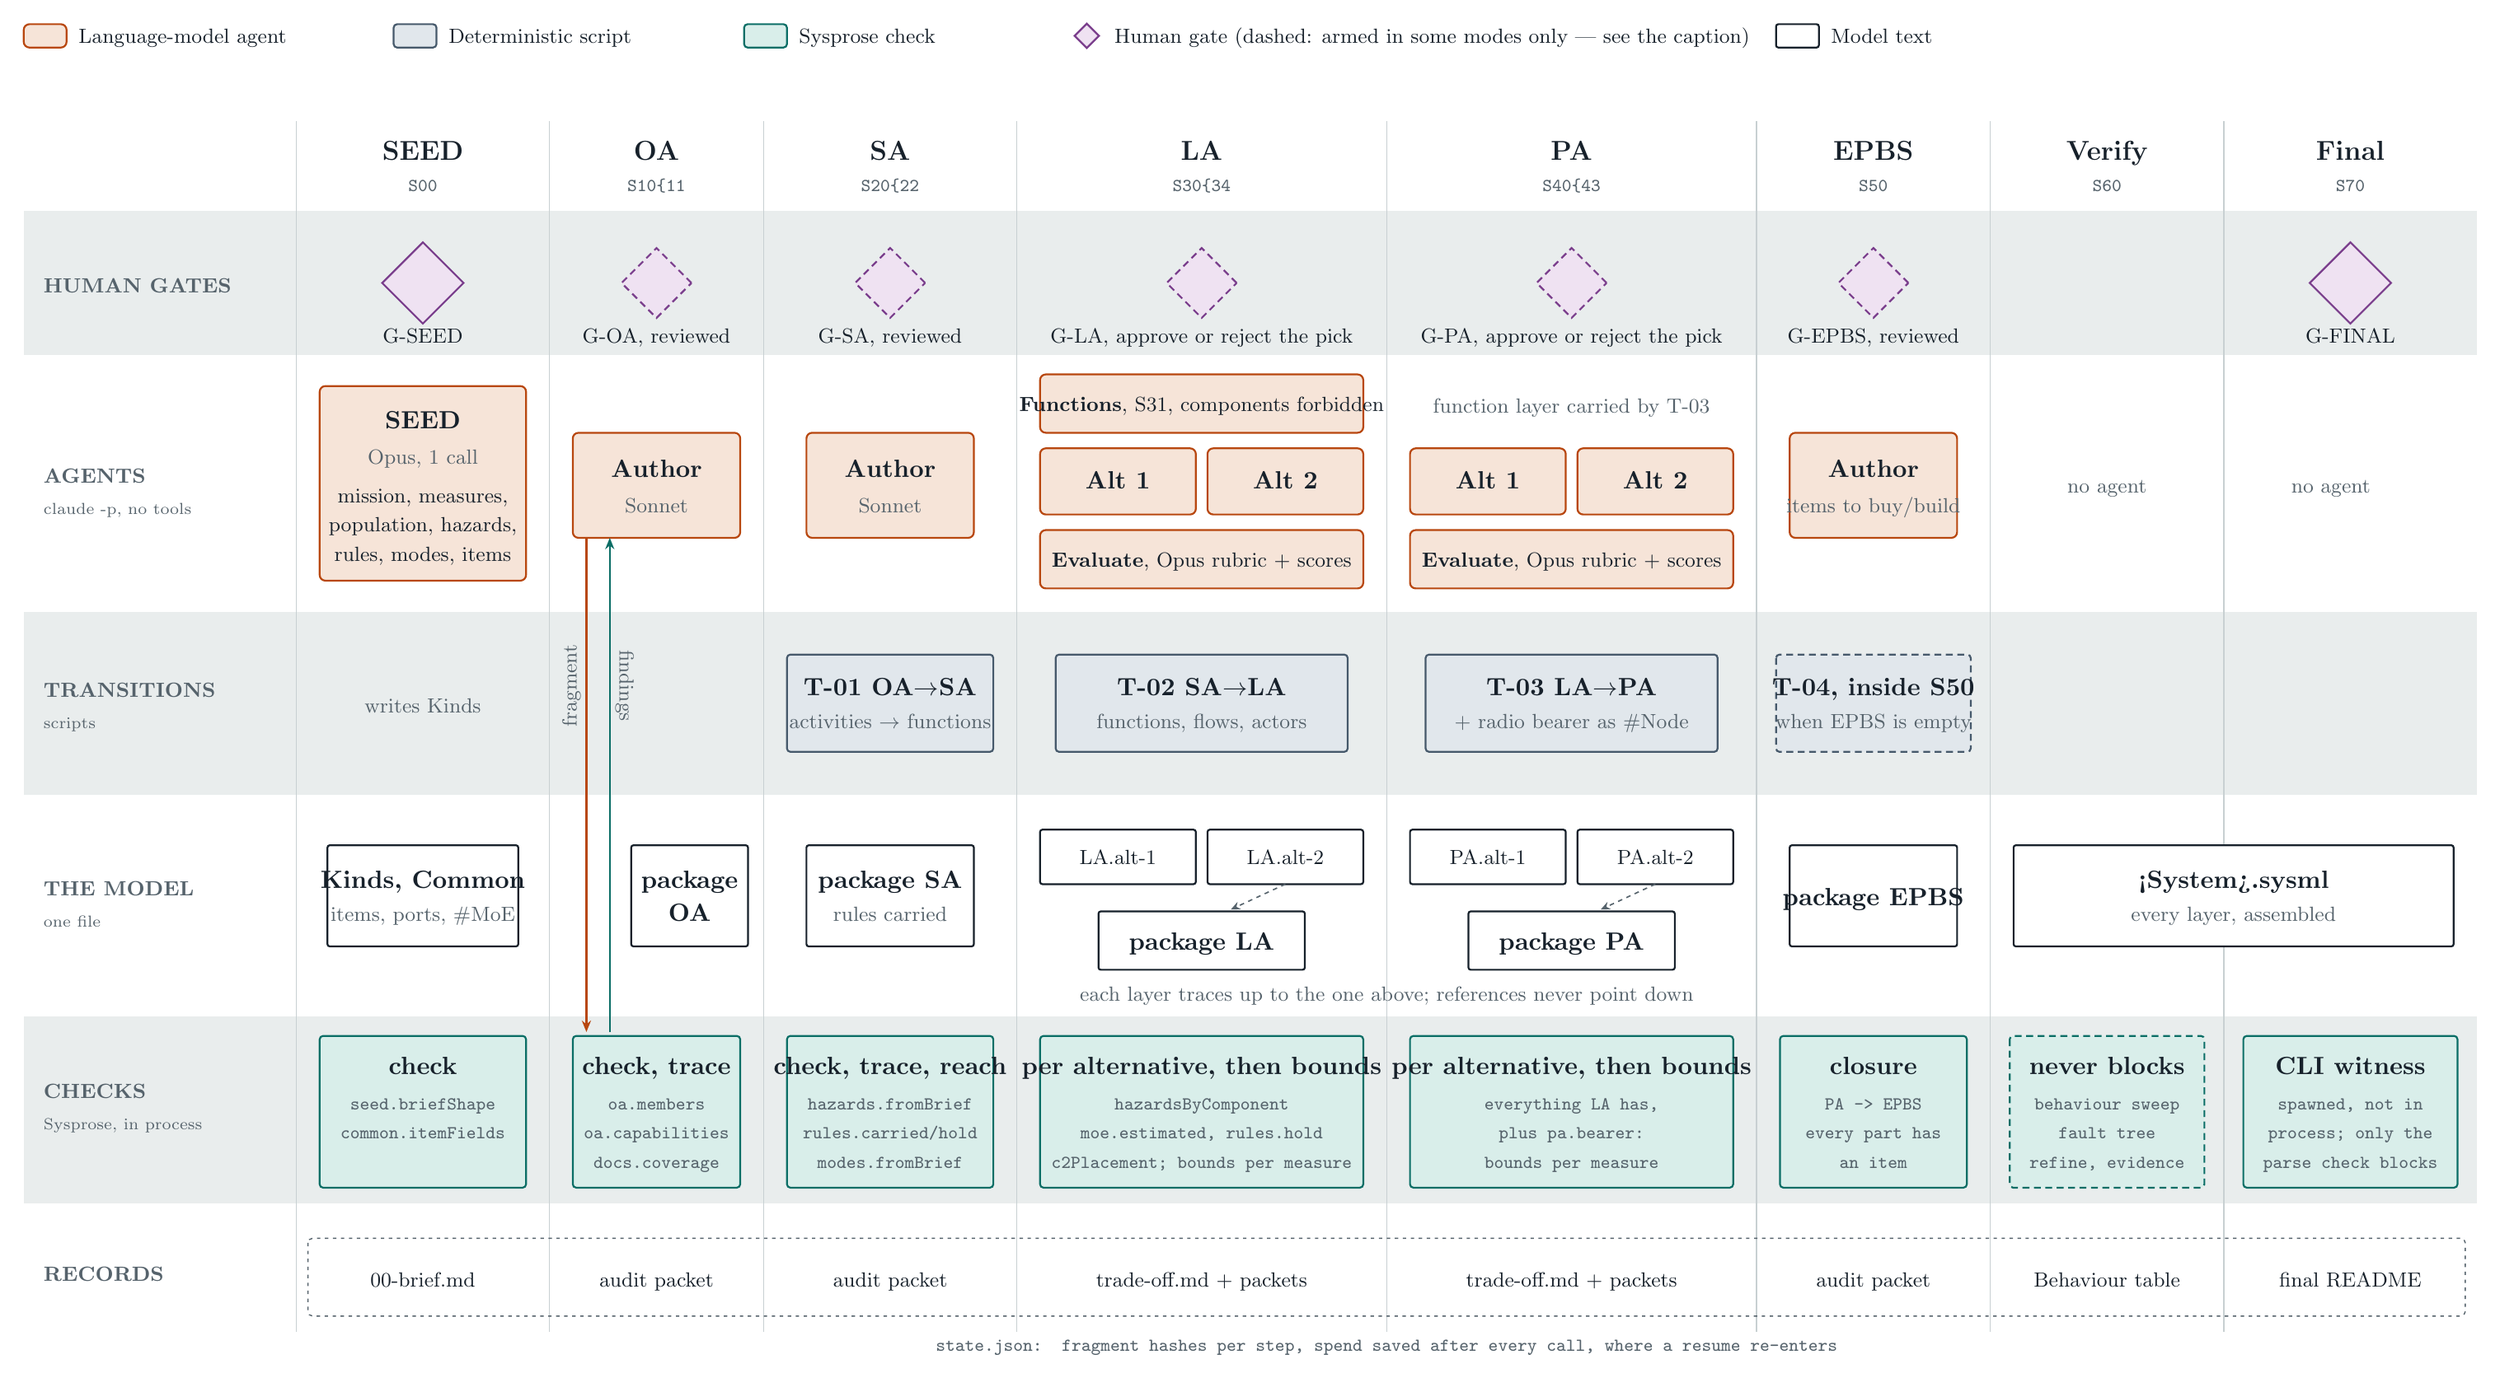
\begin{tikzpicture}[px]
  % legend
  \draw[agent] (0,-40) rectangle (22,-28); \node[tl] at (28,-30) {Language-model agent};
  \draw[script] (190,-40) rectangle (212,-28); \node[tl] at (218,-30) {Deterministic script};
  \draw[check] (370,-40) rectangle (392,-28); \node[tl] at (398,-30) {Sysprose check};
  \node[gate=11pt] at (546,-34) {}; \node[tl] at (560,-30) {Human gate (dashed: armed in some modes only --- see the caption)};
  \draw[model] (900,-40) rectangle (922,-28); \node[tl] at (928,-30) {Model text};

  % bands
  \fill[faint] (0,56) rectangle (1260,130);
  \fill[faint] (0,262) rectangle (1260,356);
  \fill[faint] (0,470) rectangle (1260,566);
  \node[band] at (10,98) {HUMAN GATES};
  \node[band] at (10,196) {AGENTS};
  \node[bandsub] at (10,212) {claude -p, no tools};
  \node[band] at (10,306) {TRANSITIONS};
  \node[bandsub] at (10,322) {scripts};
  \node[band] at (10,408) {THE MODEL};
  \node[bandsub] at (10,424) {one file};
  \node[band] at (10,512) {CHECKS};
  \node[bandsub] at (10,528) {Sysprose, in process};
  \node[band] at (10,606) {RECORDS};

  % column rules
  \foreach \x in {140,270,380,510,700,890,1010,1130} \draw[rule, line width=0.5pt] (\x,10) -- (\x,632);

  % column heads
  \foreach \x/\n/\s in {205/SEED/S00, 325/OA/S10–11, 445/SA/S20–22, 605/LA/S30–34, 795/PA/S40–43, 950/EPBS/S50, 1070/Verify/S60, 1195/Final/S70} {
    \node[th] at (\x,30) {\n};
    \node[tmono] at (\x,46) {\s};
  }

  % human gates
  \node[gate] at (205,93) {};                 \node[t] at (205,124) {G-SEED};
  \node[gatedash] at (325,93) {};             \node[t] at (325,124) {G-OA, reviewed};
  \node[gatedash] at (950,93) {};             \node[t] at (950,124) {G-EPBS, reviewed};
  \node[gatedash] at (445,93) {};             \node[t] at (445,124) {G-SA, reviewed};
  \node[gatedash] at (605,93) {};             \node[t] at (605,124) {G-LA, approve or reject the pick};
  \node[gatedash] at (795,93) {};             \node[t] at (795,124) {G-PA, approve or reject the pick};
  \node[gate] at (1195,93) {};                \node[t] at (1195,124) {G-FINAL};

  % agents
  \draw[agent] (152,146) rectangle (258,246);
  \node[tb] at (205,168) {SEED};
  \node[tmu] at (205,186) {Opus, 1 call};
  \node[t] at (205,206) {mission, measures,};
  \node[t] at (205,221) {population, hazards,};
  \node[t] at (205,236) {rules, modes, items};

  \draw[agent] (282,170) rectangle (368,224); \node[tb] at (325,193) {Author}; \node[tmu] at (325,211) {Sonnet};
  \draw[agent] (402,170) rectangle (488,224); \node[tb] at (445,193) {Author}; \node[tmu] at (445,211) {Sonnet};

  \draw[agent] (522,140) rectangle (688,170); \node[t] at (605,159) {\textbf{Functions}, S31, components forbidden};
  \draw[agent] (522,178) rectangle (602,212); \node[tb] at (562,199) {Alt 1};
  \draw[agent] (608,178) rectangle (688,212); \node[tb] at (648,199) {Alt 2};
  \draw[agent] (522,220) rectangle (688,250); \node[t] at (605,239) {\textbf{Evaluate}, Opus rubric + scores};

  \node[tmu] at (795,160) {function layer carried by T-03};
  \draw[agent] (712,178) rectangle (792,212); \node[tb] at (752,199) {Alt 1};
  \draw[agent] (798,178) rectangle (878,212); \node[tb] at (838,199) {Alt 2};
  \draw[agent] (712,220) rectangle (878,250); \node[t] at (795,239) {\textbf{Evaluate}, Opus rubric + scores};

  \draw[agent] (907,170) rectangle (993,224); \node[tb] at (950,193) {Author}; \node[tmu] at (950,211) {items to buy/build};

  \node[tmu] at (1070,201) {no agent};
  \node[tmu] at (1185,201) {no agent};

  % transitions
  \node[tmu] at (205,314) {writes Kinds};
  \draw[script] (392,284) rectangle (498,334); \node[tb] at (445,305) {T-01 OA$\to$SA}; \node[tmu] at (445,322) {activities $\to$ functions};
  \draw[script] (530,284) rectangle (680,334); \node[tb] at (605,305) {T-02 SA$\to$LA}; \node[tmu] at (605,322) {functions, flows, actors};
  \draw[script] (720,284) rectangle (870,334); \node[tb] at (795,305) {T-03 LA$\to$PA}; \node[tmu] at (795,322) {+ radio bearer as \#Node};
  % T-04 is not a step: S50 seeds itself with it when EPBS is still empty.
  \draw[script, dash pattern=on 3pt off 2pt] (900,284) rectangle (1000,334); \node[tb] at (950,305) {T-04, inside S50}; \node[tmu] at (950,322) {when EPBS is empty};

  % model
  \draw[model] (156,382) rectangle (254,434); \node[tb] at (205,404) {Kinds, Common}; \node[tmu] at (205,421) {items, ports, \#MoE};
  \draw[model] (312,382) rectangle (372,434); \node[tb] at (342,404) {package}; \node[tb] at (342,421) {OA};
  \draw[model] (402,382) rectangle (488,434); \node[tb] at (445,404) {package SA}; \node[tmu] at (445,421) {rules carried};
  \draw[model] (522,374) rectangle (602,402); \node[t] at (562,392) {LA.alt-1};
  \draw[model] (608,374) rectangle (688,402); \node[t] at (648,392) {LA.alt-2};
  \draw[model] (552,416) rectangle (658,446); \node[tb] at (605,436) {package LA};
  \draw[flowfaint] (648,402) -- (620,415);
  \draw[model] (712,374) rectangle (792,402); \node[t] at (752,392) {PA.alt-1};
  \draw[model] (798,374) rectangle (878,402); \node[t] at (838,392) {PA.alt-2};
  \draw[model] (742,416) rectangle (848,446); \node[tb] at (795,436) {package PA};
  \draw[flowfaint] (838,402) -- (810,415);
  \draw[model] (907,382) rectangle (993,434); \node[tb] at (950,413) {package EPBS};
  \draw[model] (1022,382) rectangle (1248,434); \node[tb] at (1135,404) {<System>.sysml}; \node[tmu] at (1135,421) {every layer, assembled};
  \node[tmu] at (700,462) {each layer traces up to the one above; references never point down};

  % author <-> check, shown once per authoring step
  \draw[flowagent] (289,224) -- (289,478);
  \draw[flowcheck] (301,478) -- (301,224);
  \node[tmu, rotate=90, anchor=base] at (284,300) {fragment};
  \node[tmu, rotate=-90, anchor=base] at (306,300) {findings};

  % checks
  \draw[check] (152,480) rectangle (258,558);
  \node[tb] at (205,500) {check}; \node[tmono] at (205,518) {seed.briefShape}; \node[tmono] at (205,533) {common.itemFields};
  \draw[check] (282,480) rectangle (368,558);
  \node[tb] at (325,500) {check, trace}; \node[tmono] at (325,518) {oa.members}; \node[tmono] at (325,533) {oa.capabilities}; \node[tmono] at (325,548) {docs.coverage};
  \draw[check] (392,480) rectangle (498,558);
  \node[tb] at (445,500) {check, trace, reach}; \node[tmono] at (445,518) {hazards.fromBrief}; \node[tmono] at (445,533) {rules.carried/hold}; \node[tmono] at (445,548) {modes.fromBrief};
  \draw[check] (522,480) rectangle (688,558);
  \node[tb] at (605,500) {per alternative, then bounds}; \node[tmono] at (605,518) {hazardsByComponent}; \node[tmono] at (605,533) {moe.estimated, rules.hold}; \node[tmono] at (605,548) {c2Placement; bounds per measure};
  \draw[check] (712,480) rectangle (878,558);
  \node[tb] at (795,500) {per alternative, then bounds}; \node[tmono] at (795,518) {everything LA has,}; \node[tmono] at (795,533) {plus pa.bearer:}; \node[tmono] at (795,548) {bounds per measure};
  \draw[check] (902,480) rectangle (998,558);
  \node[tb] at (950,500) {closure}; \node[tmono] at (950,518) {PA -> EPBS}; \node[tmono] at (950,533) {every part has}; \node[tmono] at (950,548) {an item};
  \draw[check, dash pattern=on 3pt off 2pt] (1020,480) rectangle (1120,558);
  \node[tb] at (1070,500) {never blocks}; \node[tmono] at (1070,518) {behaviour sweep}; \node[tmono] at (1070,533) {fault tree}; \node[tmono] at (1070,548) {refine, evidence};
  \draw[check] (1140,480) rectangle (1250,558);
  \node[tb] at (1195,500) {CLI witness}; \node[tmono] at (1195,518) {spawned, not in}; \node[tmono] at (1195,533) {process; only the}; \node[tmono] at (1195,548) {parse check blocks};

  % records
  \draw[record] (146,584) rectangle (1254,624);
  \foreach \x/\r in {205/00-brief.md, 325/audit packet, 445/audit packet, 605/trade-off.md + packets, 795/trade-off.md + packets, 950/audit packet, 1070/Behaviour table, 1195/final README}
    \node[t] at (\x,609) {\r};
  \node[tmono] at (700,642) {state.json: fragment hashes per step, spend saved after every call, where a resume re-enters};
\end{tikzpicture}

\captionof{figure}{\textbf{Six bands of responsibility against the twenty steps} (S01 and S02, the optional intake lanes, are off by default and not drawn). Orange boxes are the only places a language model runs; at LA and PA it writes two architectures on the same carried function layer and an evaluator picks one. The paired arrows at OA stand for every authoring step: the fragment goes down to the checks, the findings come back up. A step that still blocks after three repair rounds \emph{stops the run}; it opens its gate first only where a gate exists (S00, S10, S21, S33, S42, S50, S70 — the transitions and the two alternatives steps have none), and approving that gate records the decision and stops too. The way on is an edit and a \texttt{resume}. Solid gates are armed in every mode, but \texttt{-{}-unattended} takes them automatically: in v7 both were.}

\newpage
% ───────────────────────────── Figure 2 ─────────────────────────────
{\fontsize{18}{22}\selectfont\bfseries One alternative-authoring step, up close}\par\smallskip
{\color{muted}S32 and S41, where the model writes one of two architectures. The model never touches a file: what it returns is composed onto the fixed function layer, assembled with the layers above, and checked before anything is kept. A plain author — S10, S21, S31, S50 — runs the same loop without the Compose stage.}\par\bigskip

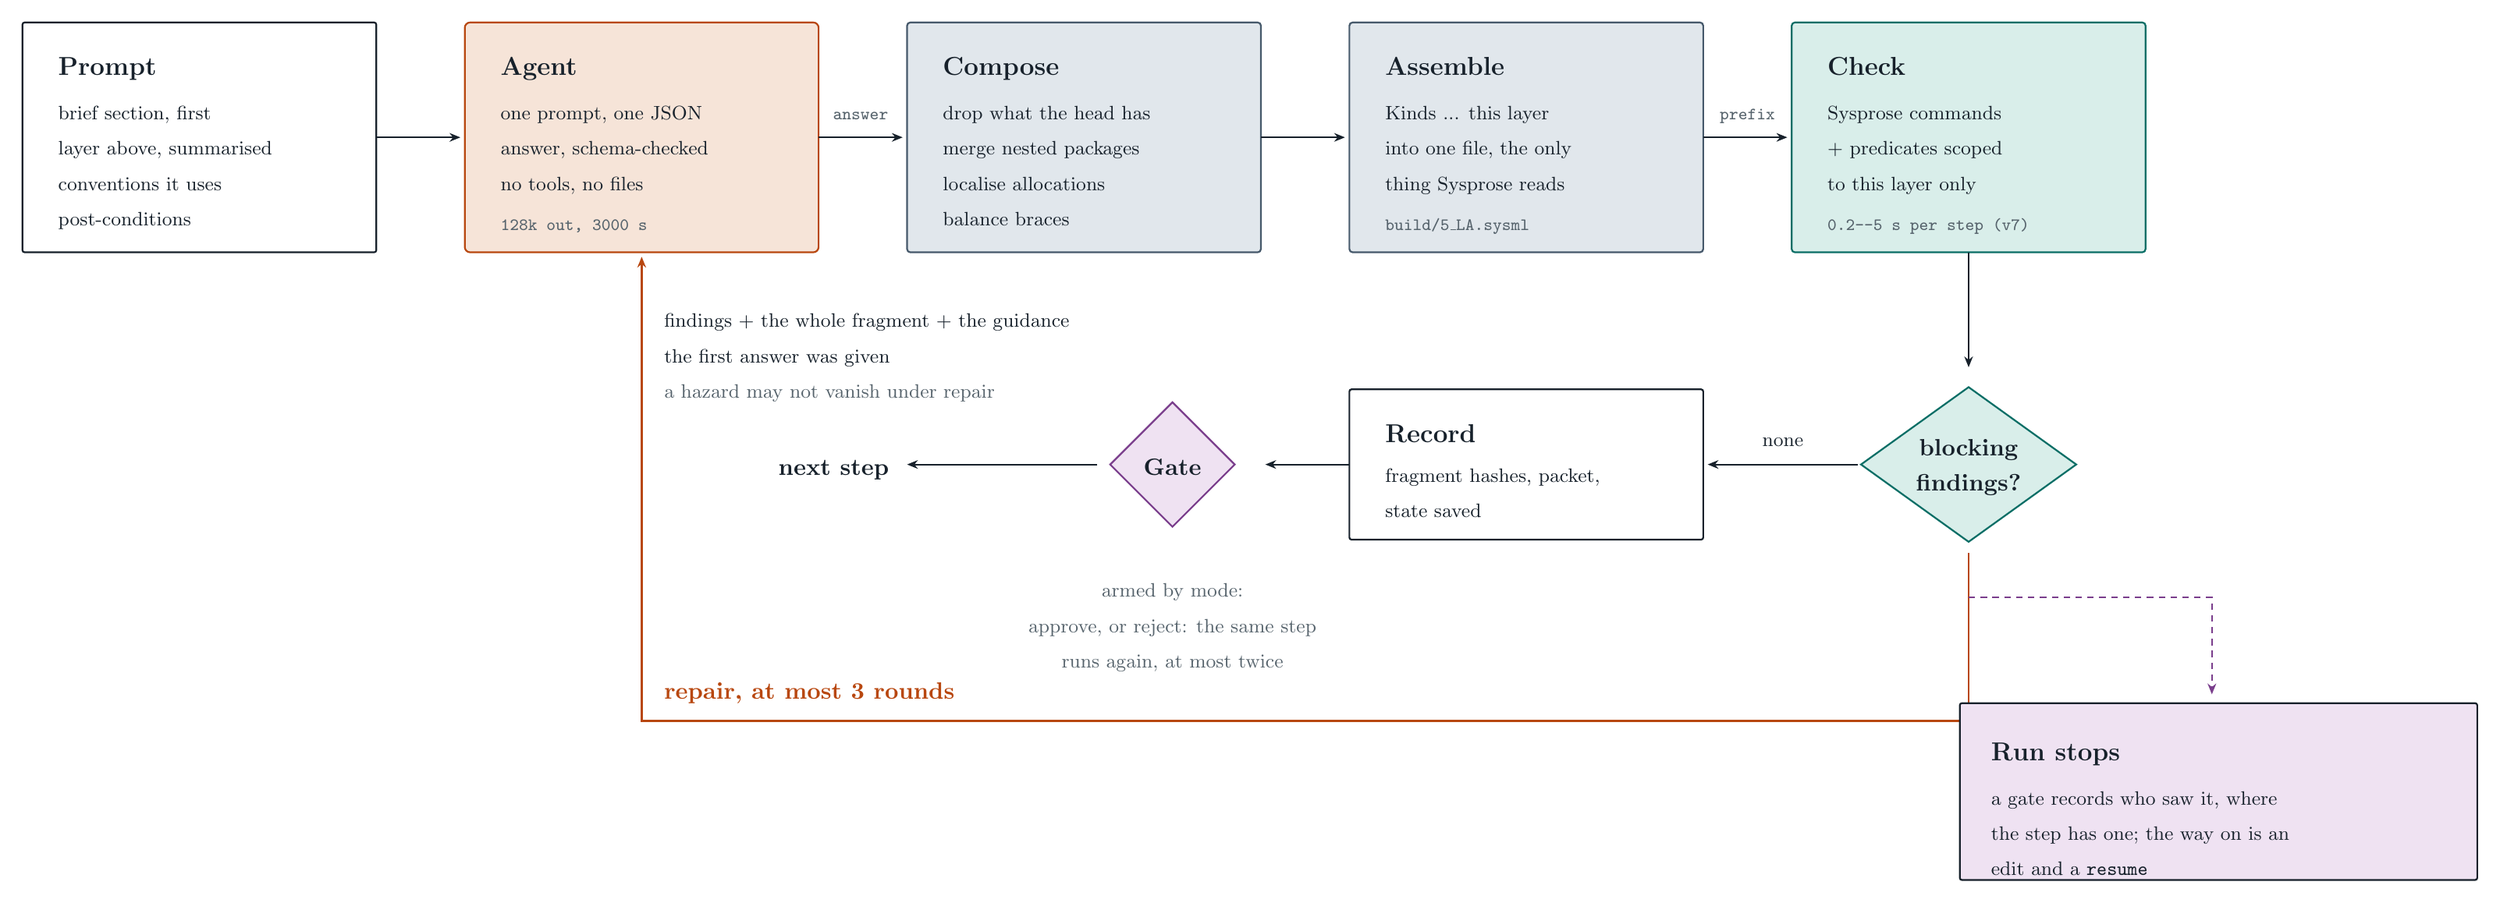
\begin{tikzpicture}[x=0.036cm, y=-0.036cm]
  \draw[model] (20,40) rectangle (180,144);
  \node[thl] at (36,64) {Prompt}; \node[tl] at (36,84) {brief section, first}; \node[tl] at (36,100) {layer above, summarised}; \node[tl] at (36,116) {conventions it uses}; \node[tl] at (36,132) {post-conditions};

  \draw[agent] (220,40) rectangle (380,144);
  \node[thl] at (236,64) {Agent}; \node[tl] at (236,84) {one prompt, one JSON}; \node[tl] at (236,100) {answer, schema-checked}; \node[tl] at (236,116) {no tools, no files}; \node[tmonol] at (236,134) {128k out, 3000 s};

  \draw[script] (420,40) rectangle (580,144);
  \node[thl] at (436,64) {Compose}; \node[tl] at (436,84) {drop what the head has}; \node[tl] at (436,100) {merge nested packages}; \node[tl] at (436,116) {localise allocations}; \node[tl] at (436,132) {balance braces};

  \draw[script] (620,40) rectangle (780,144);
  \node[thl] at (636,64) {Assemble}; \node[tl] at (636,84) {Kinds ... this layer}; \node[tl] at (636,100) {into one file, the only}; \node[tl] at (636,116) {thing Sysprose reads}; \node[tmonol] at (636,134) {build/5\_LA.sysml};

  \draw[check] (820,40) rectangle (980,144);
  \node[thl] at (836,64) {Check}; \node[tl] at (836,84) {Sysprose commands}; \node[tl] at (836,100) {+ predicates scoped}; \node[tl] at (836,116) {to this layer only}; \node[tmonol] at (836,134) {0.2--5 s per step (v7)};

  \draw[flow] (180,92) -- (218,92);
  \draw[flow] (380,92) -- (418,92);
  \draw[flow] (580,92) -- (618,92);
  \draw[flow] (780,92) -- (818,92);
  \node[tmono] at (399,84) {answer};
  \node[tmono] at (800,84) {prefix};

  \draw[flow] (900,144) -- (900,196);
  \node[diamond, draw=check, fill=checkTint, line width=0.8pt, minimum width=100pt, minimum height=72pt, inner sep=0pt] at (900,240) {};
  \node[tb] at (900,236) {blocking};
  \node[tb] at (900,252) {findings?};

  \draw[flow] (850,240) -- (782,240);
  \node[t] at (816,232) {none};
  \draw[model] (620,206) rectangle (780,274);
  \node[thl] at (636,230) {Record}; \node[tl] at (636,248) {fragment hashes, packet,}; \node[tl] at (636,264) {state saved};
  \draw[flow] (620,240) -- (582,240);
  \node[gate=58pt] at (540,240) {};
  \node[tb] at (540,245) {Gate};
  \node[tmu] at (540,300) {armed by mode:};
  \node[tmu] at (540,316) {approve, or reject: the same step};
  \node[tmu] at (540,332) {runs again, at most twice};
  \draw[flow] (506,240) -- (420,240);
  \node[tb, anchor=base east] at (412,245) {next step};

  \draw[flowagent] (900,280) -- (900,356) -- (300,356) -- (300,146);
  \node[tb, anchor=base west, text=agent] at (310,346) {repair, at most 3 rounds};
  \node[tl] at (310,178) {findings + the whole fragment + the guidance};
  \node[tl] at (310,194) {the first answer was given};
  \node[tmul] at (310,210) {a hazard may not vanish under repair};
  % Round 3 does not hand over to the gate chain: the run stops.
  \draw[flowhuman] (900,300) -- (1010,300) -- (1010,344);
  \draw[model, fill=humanTint] (896,348) rectangle (1130,428);
  \node[thl] at (910,374) {Run stops};
  \node[tl] at (910,394) {a gate records who saw it, where};
  \node[tl] at (910,410) {the step has one; the way on is an};
  \node[tl] at (910,426) {edit and a \texttt{resume}};
\end{tikzpicture}

\captionof{figure}{\textbf{One alternative-authoring step (S32, S41); the model writes, it never edits files.} Compose is this step's own: a plain author (S10, S21, S31, S50) has its carried trace and allocate lines restored and its answer preflighted instead. A diagnostic anchored in a layer above is reported, not sent back — the author cannot change that layer — and travels on as a note. A blocking finding goes back with the fragment it came from, at most three times; after that the run stops. Check times: 0.2--5\,s per step's checks in v7.}

\newpage
% ───────────────────────────── Figure 3 ─────────────────────────────
{\fontsize{18}{22}\selectfont\bfseries Two architectures, one choice}\par\smallskip
{\color{muted}At LA and PA the functions are fixed and shared, so only the split of responsibilities differs. The two alternatives are built to disagree on where coordination and command live, and the score says what that costs.}\par\bigskip

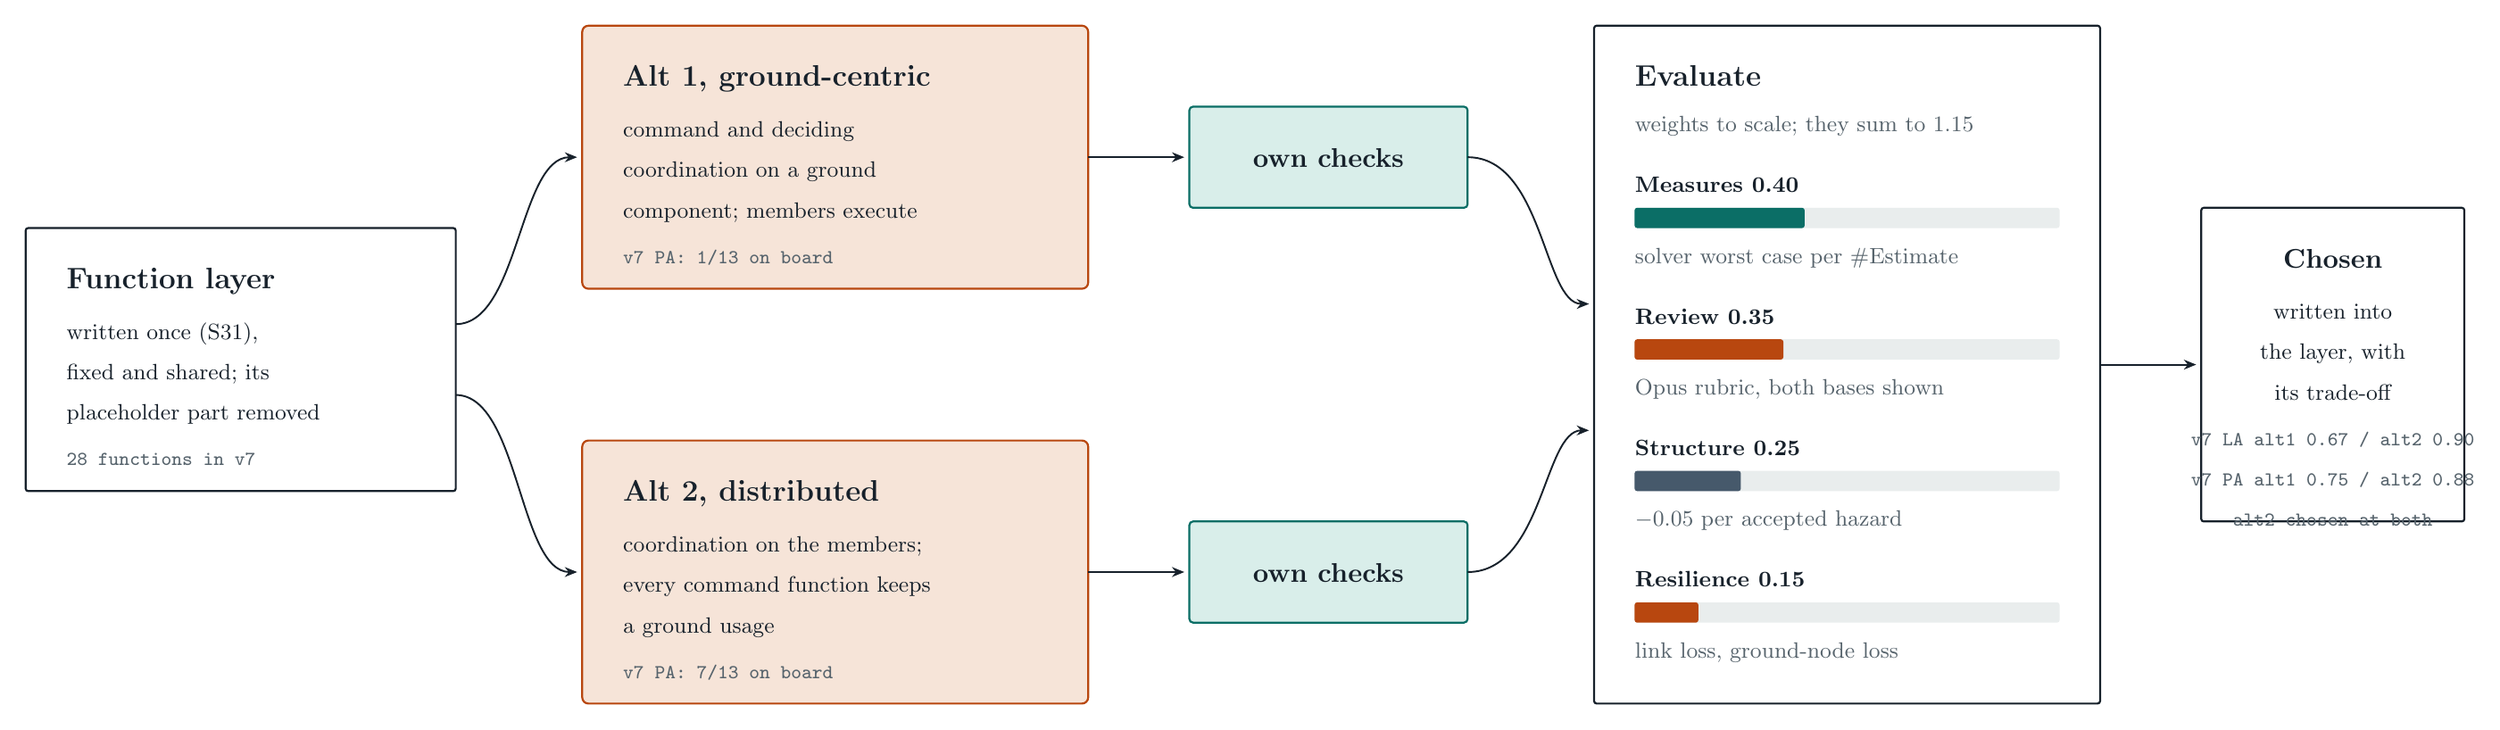
\begin{tikzpicture}[x=0.036cm, y=-0.036cm]
  \draw[model] (20,120) rectangle (190,224);
  \node[thl] at (36,144) {Function layer}; \node[tl] at (36,164) {written once (S31),}; \node[tl] at (36,180) {fixed and shared; its}; \node[tl] at (36,196) {placeholder part removed}; \node[tmonol] at (36,214) {28 functions in v7};

  \draw[agent] (240,40) rectangle (440,144);
  \node[thl] at (256,64) {Alt 1, ground-centric}; \node[tl] at (256,84) {command and deciding}; \node[tl] at (256,100) {coordination on a ground}; \node[tl] at (256,116) {component; members execute}; \node[tmonol] at (256,134) {v7 PA: 1/13 on board};

  \draw[agent] (240,204) rectangle (440,308);
  \node[thl] at (256,228) {Alt 2, distributed}; \node[tl] at (256,248) {coordination on the members;}; \node[tl] at (256,264) {every command function keeps}; \node[tl] at (256,280) {a ground usage}; \node[tmonol] at (256,298) {v7 PA: 7/13 on board};

  \draw[flow] (190,158) .. controls (215,158) and (215,92) .. (238,92);
  \draw[flow] (190,186) .. controls (215,186) and (215,256) .. (238,256);

  \draw[check] (480,72) rectangle (590,112); \node[tb] at (535,96) {own checks};
  \draw[check] (480,236) rectangle (590,276); \node[tb] at (535,260) {own checks};
  \draw[flow] (440,92) -- (478,92);
  \draw[flow] (440,256) -- (478,256);
  \draw[flow] (590,92) .. controls (620,92) and (620,150) .. (638,150);
  \draw[flow] (590,256) .. controls (620,256) and (620,200) .. (638,200);

  % evaluator; bars drawn to scale, 1.00 = 168 units
  \draw[model] (640,40) rectangle (840,308);
  \node[thl] at (656,64) {Evaluate};
  \node[tmul] at (656,82) {weights to scale; they sum to 1.15};
  \foreach \y/\lab/\w/\col/\note in {
      106/Measures 0.40/67.2/check/solver worst case per \#Estimate,
      158/Review 0.35/58.8/agent/Opus rubric{,} both bases shown,
      210/Structure 0.25/42/script/$-$0.05 per accepted hazard,
      262/Resilience 0.15/25.2/agent/link loss{,} ground-node loss} {
    \node[tl, font=\fontsize{9}{11}\selectfont\bfseries] at (656,\y) {\lab};
    \fill[faint, rounded corners=1pt] (656,\y+6) rectangle (824,\y+14);
    \fill[fill=\col, rounded corners=1pt] (656,\y+6) rectangle ({656+\w},\y+14);
    \node[tmul] at (656,\y+28) {\note};
  }

  \draw[flow] (840,174) -- (878,174);
  \draw[model] (880,112) rectangle (984,236);
  \node[tb] at (932,136) {Chosen}; \node[t] at (932,156) {written into}; \node[t] at (932,172) {the layer, with}; \node[t] at (932,188) {its trade-off};
  \node[tmono] at (932,206) {v7 LA alt1 0.67 / alt2 0.90}; \node[tmono] at (932,222) {v7 PA alt1 0.75 / alt2 0.88}; \node[tmono] at (932,238) {alt2 chosen at both};
\end{tikzpicture}

\captionof{figure}{\textbf{A measure decides only when some alternative misses it.} Each estimate is the architecture's own claim, bounded for its worst case; totals run to 1.15, not 1, because the four weights are not normalised. The final audit lists the targets every alternative met: in v7, 12 of 14. Without a population the resilience criteria are not judged and every alternative takes a neutral 0.5; the ground-centric/distributed split is a population rule, and if one alternative fails its checks the other is taken with no comparison.}

\end{document}
